\documentclass[twoside,twocolumn,usenatbib]{mnras}

\usepackage{graphicx}
\usepackage{amsmath}
\usepackage{amssymb}
\usepackage{booktabs}

% --------------------------------------------------------------- title data --
\title[Coordination Without a Coordinator]{Coordination Without a Coordinator:
  A Scientific Programme for Hormone-Inspired Residual-Demand Signalling}

\author[Tilanthi]{Tilanthi\\
BIODISC --- Biology Discovery and Intelligence System}
\date{Accepted XXX. Received YYY; in original form ZZZ}

\begin{document}
\label{firstpage}
\pagerange{\pageref{firstpage}--\pageref{lastpage}}

\maketitle

\begin{abstract}
How much must a node know, and what must a shared medium provide, for $n$
minimally-informed autonomous agents to produce a specified global behaviour
--- reliably, terminably, and with coordination cost carried by an explicit
five-component vector (agent and medium communication, agent and medium
state, latency; the agent-side component $O(n\,k)$ with $k \ll n$,
conditional on a medium providing broadcast, locality and decay)
--- with no central coordinator? Mammalian wound healing is an existence
proof over a substantial operating envelope: a wound is repaired by cells
that perceive only local chemistry plus built-in capability, organised
end-to-end by broadcast signals that receivers interpret, with production
of new responders ramped by the unconsumed remainder of a constitutive
signal. We distil this reference system into five coordination primitives
--- receiver-defined meaning, concentration-as-instruction,
residual-signal-as-demand, co-stimulus guards, antagonist termination ---
plus one separated architectural assumption (cheap responders, elastic
factories), and find that the sixteen families we survey jointly fail
to cover them, the residual-signal demand loop above all. We derive the
central law's equilibria and its delay-stability threshold, demonstrate
its fibrotic failure mode in simulation, and lay out
a five-phase programme --- controller analysis, factorial ablation
sandbox, benchmarks and inverse design, substrate engineering, and
failure theory mapping the operating boundary --- with falsifiable
predictions and stated criteria per phase (a termination criterion for
the core mechanism, claim-reducing criteria elsewhere), testing three
separable hypotheses: mechanistic, architectural, and comparative.
The medium is not free, and whether the coordinator has merely been
hidden inside it is a criterion the programme itself tests, not an
assumption.
\end{abstract}

\begin{keywords}
distributed systems --- self-organization --- bio-inspired computing ---
amorphous computing --- wound healing --- autonomous systems
\end{keywords}

\section{Introduction}

\label{sec:intro}

This paper is organised around one basic question:

\begin{quote}
\emph{How much must a node know, and what must a shared medium provide, for
$n$ minimally-informed autonomous agents to produce a specified global
behaviour --- reliably, terminably, and at communication cost $O(n\,k)$
with $k \ll n$ --- with no central coordinator?}
\end{quote}

The premise hiding in the question is economic. If every agent must
coordinate with every other, coordination state grows as $O(n^2)$ and
compounds with growth. If each agent holds only local state and reacts to
signals by built-in capability, a disturbance involving $k$ agents costs
roughly $O(n\,k)$ in signalling, and adding an agent adds capacity
rather than coordination load. The premise is not free: it requires a
medium providing broadcast with locality and decay, and it restricts
which behaviours are reachable; the programme makes those requirements
precise. The paper's cost statement is accordingly a five-component
vector --- agent and medium communication, agent and medium state,
latency --- of which $O(n\,k)$ is only the agent-communication
component; the medium's share is a real cost paid in Phase~IV, not an
idealisation. One distinction organises everything that follows:
what is decentralised is \emph{decision-making and knowledge}, not
necessarily physical plant --- factories may be centralised and media
shared; the argument is against centralised \emph{deciding}, not against
shared infrastructure (Section~\ref{sec:discussion}).

Biology answers the question once, in tissue repair. Exposed blood
triggers thrombin, which polymerises fibrin and traps red cells into a
mat that stops the bleeding --- local chemistry, no coordinator. Damaged
cells release stress signals that recruit neutrophils and macrophages to
clear contamination \citep{medzhitov2008}. If local responders are
insufficient, the unconsumed remainder of the hormone thrombopoietin
accumulates in plasma and ramps platelet
production in the marrow \citep{kaushansky2005}; G-CSF runs a related,
further-layered programme for neutrophils under severe demand
\citep{manz2014}. Every cell does what it
is programmed to do; signals arrive with the blood; the wound closes.
The same mechanism operates from pinprick to major trauma --- though
overwhelming injury does break it, a boundary the programme must map
rather than assume away \citep{gurtner2008}.

We propose to treat this as more than an analogy: read wound healing as
an \emph{engineering specification} that evolution has stress-tested ---
robust across a substantial envelope, though neither optimal nor
pathology-free --- extract its coordination principles
(Section~\ref{sec:wound}), and
subject them to the scrutiny any competing architecture would face
(Section~\ref{sec:programme}); Fig.~\ref{fig:arch} contrasts the two
architectures.

\begin{figure}
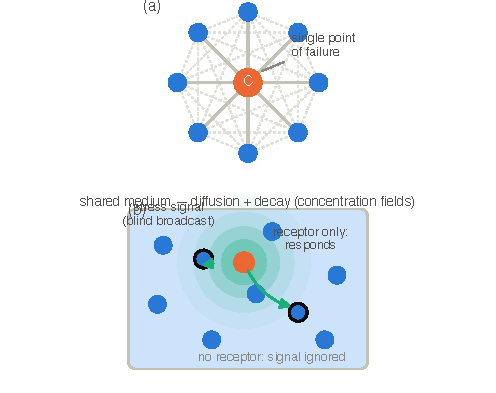
\includegraphics[width=\columnwidth]{fig1_architecture}
\caption{Two coordination architectures. (a) Central orchestration: the hub
holds $O(n)$ state and pairwise traffic grows as $O(n^2)$; the hub is a
single point of failure. (b) A hormonal medium: a stressed agent emits a
signal that diffuses and decays; only receptor-equipped agents respond.
Every agent holds $O(1)$ state; a disturbance reaching $k$ receivers costs
$O(n\,k)$ messages. Meaning lives in the receiver.}
\label{fig:arch}
\end{figure}

The contributions are: (i) a precise statement of the coordinator-free
coordination question, with the five-component cost vector (agent and
medium communication, agent and medium state, latency) as the primary
complexity claim, of which $O(n\,k)$ is the agent-side component;
(ii) a five-primitive distillation of wound healing plus one separated
architectural assumption, with its pathologies (cytokine storm,
thrombosis, autoimmunity, fibrosis) read as engineering safeguards;
(iii) a gap analysis showing the sixteen families surveyed jointly
fail to cover the primitives --- the residual-signal
demand loop absent from all of them; and (iv) a five-phase programme with
falsifiable predictions and a stated criterion per phase --- terminal
for the core mechanism, claim-reducing elsewhere --- organised
around three hypotheses that can fail independently
(Section~\ref{sec:programme}). This is a
research-programme paper: it reports an equilibrium and stability
analysis of the central control law and one illustrative simulation
(Fig.~\ref{fig:loop}), and a falsifiable plan --- not
completed experiments; Phase~II onward is where the predictions are
tested. The predictions, effect sizes and kill criteria are written to
be registrable: a Perspective or Stage-1 registered-report track is the
intended submission form.

\section{Prior approaches}
\label{sec:prior}

\subsection{Central orchestration, autonomic and control-theoretic
computing}

The dominant engineering answer is a coordinator: cluster managers such
as Borg and Kubernetes concentrate placement, scaling and failure
handling at a (replicated) control plane \citep{burns2016}, autonomic
computing envisioned managed systems reporting to an external control
loop \citep{kephart2003}, and control-theoretic computing designs
classical feedback controllers against measured metrics
\citep{hellerstein2004}. These work at
impressive scale, but the coordination is bought: global state, global
visibility, superlinear traffic. The modern ecosystem --- service-mesh
sidecars, event-driven autoscaling, chaos engineering --- refines this
pipeline without changing its epistemics: the error signal is still
measured and reported, never physical. The impossibility result of
\citet{fischer1985} --- consensus with one faulty process is unsolvable
asynchronously --- directed a large literature towards tolerating
coordinators rather than eliminating them. Our question is orthogonal: not how to make a coordinator
fault-tolerant, but which global behaviours need none.

\subsection{Named communication: tuple spaces, actors, pub/sub, gossip}

Linda's tuple spaces decouple senders from receivers: writers publish,
receivers select by template \citep{carriero1989}; the actor model
locates meaning in the receiver's handling \citep{agha1986};
publish--subscribe and epidemic protocols \citep{demers1987} push
receiver-side selection to Internet scale. These families anticipate our first principle, but the medium
carries \emph{identity}, not \emph{concentration}: a message is
delivered or not, it does not accumulate into a graded, decaying field,
and nothing in the medium encodes demand.

\subsection{Stigmergy and quorum sensing}

Stigmergy --- ants laying and following evaporating pheromone trails ---
is the closest biological precedent in computing, formalised as indirect
coordination through environment modification \citep{parunak1997,
dorigo1996}. Bacterial quorum sensing is its concentration-threshold
cousin: cells secrete an autoinducer and switch behaviour above a
threshold \citep{miller2001}. Both give concentration
semantics with decay, but the repertoire answers ``how many of us are
here?'', not ``who needs help, and is supply keeping up?'' --- and the
limits of that repertoire are now measured directly, not merely
asserted, in high-density pheromone-swarm robotics \citep{hunt2019}.

\subsection{Amorphous computing and synthetic pattern formation}

Amorphous computing asked exactly our question for programmable matter:
what global shapes can unreliable, identical, locally-communicating
particles achieve \citep{abelson2000}? Gradient and threshold
primitives were compiled into global behaviours \citep{nagpal2003}, and
synthetic biology realised them in living cells --- pattern formation
from diffusing signals \citep{basu2005}, population control with an
explicit kill term \citep{you2004}. The line proves receiver-side
threshold logic on a diffusing medium can compute global structure, but
stops short of logistics: nothing ramps production by unmet demand, and
termination is programmed, not emergent.

\subsection{Field-based and hormone-inspired coordination}

The closest prior art takes hormones seriously. Field-based
coordination computes distributed gradient fields and has agents follow
them \citep{mamei2006}. The Digital Hormone Model controls
modular-robot self-organisation with hormone-like signals that diffuse,
carry concentration and decay --- the closest precedent to our P1 and
P2 \citep{shen2004}. The artificial-endocrine-system family develops
lattice models of endocrine regulation for robotic swarms, requiring no
unique identifiers or global information \citep{xu2011}, and the
Artificial Hormone System assigns real-time tasks using locally
computed ``hormones'' that rise with waiting tasks and fall with load
\citep{brinkschulte2008}. The distinction lies at P3: in these systems
the hormone is a \emph{score}, computed and consumed by nodes to guide
movement or assignment; no signal is constitutively produced and
cleared by its own consumers, so no residual encodes unmet demand, and
antagonist dissolution is not a termination primitive. Immune-inspired
systems contribute the other half of our safety story: the danger model
\citep{matzinger1994, matzinger2002} and its dendritic-cell
implementation \citep{greensmith2005} demonstrate co-stimulus gating
--- but as classifiers, not coordinators.

\subsection{The gap}

\begin{table}
\centering
\caption{Coverage of the five coordination primitives P1--P5 and the
architectural assumption A1 (Section~\ref{sec:principles}) by prior
families. \checkmark\ = native; $\sim$ = partial or incidental; --
= absent. The final row is definitional --- an internal consistency
check that the primitive set describes the reference system, not an
empirical comparison.}
\label{tab:gap}
\footnotesize
\begin{tabular}{@{}lcccccc@{}}
\toprule
Family & P1 & P2 & P3 & P4 & P5 & A1 \\
\midrule
Central orchestration & -- & -- & -- & $\sim$ & $\sim$ & \checkmark \\
Tuple spaces / actors & \checkmark & -- & -- & -- & -- & -- \\
Pub--sub / gossip & \checkmark & $\sim$ & -- & -- & $\sim$ & -- \\
Stigmergy (ants) & \checkmark & \checkmark & -- & -- & $\sim$ & \checkmark \\
Quorum sensing & \checkmark & \checkmark & -- & -- & -- & \checkmark \\
Amorphous computing & $\sim$ & \checkmark & -- & -- & $\sim$ & -- \\
Synthetic biology & \checkmark & \checkmark & -- & \checkmark & $\sim$ & \checkmark \\
Field-based coordination & \checkmark & \checkmark & $\sim$ & -- & $\sim$ & -- \\
Digital Hormone Model & \checkmark & \checkmark & -- & -- & $\sim$ & -- \\
Artificial endocrine systems & \checkmark & $\sim$ & $\sim$ & -- & $\sim$ & -- \\
Artificial Hormone System & \checkmark & $\sim$ & $\sim$ & -- & $\sim$ & -- \\
Danger theory / DCA & \checkmark & $\sim$ & -- & \checkmark & -- & -- \\
Congestion / back-pressure & -- & $\sim$ & $\sim$ & -- & $\sim$ & $\sim$ \\
Antithetic integral feedback & -- & $\sim$ & $\sim$ & -- & \checkmark & -- \\
Token-bucket / credit control & -- & $\sim$ & $\sim$ & -- & $\sim$ & $\sim$ \\
Metabolic / homeostatic & -- & $\sim$ & $\sim$ & -- & $\sim$ & -- \\
\midrule
\emph{Wound-healing class} & \checkmark & \checkmark & \checkmark & \checkmark & \checkmark & \checkmark \\
\bottomrule
\end{tabular}
\end{table}

Table~\ref{tab:gap} arranges the sixteen families against the primitives
defined below. Every family covers a proper subset; no family implements
P3, the residual-signal demand loop, natively. Four near-misses
demand honesty. Congestion control and back-pressure
\citep{kelly1998} signal demand through queue backlog --- a genuine
residual --- but the backlog is measured state reported to a computed
controller, not a constitutive blind-broadcast signal consumed by its
own responders. Antithetic integral feedback \citep{briat2016} realises
the unpaired remainder of two annihilating species as an error signal
--- inside a single well, not as a coordination medium across a fleet;
it has since been realised experimentally in living and cell-free
systems \citep{aoki2019}, a residue-as-error implementation that
remains within a single controlled volume.
Token-bucket and credit-based flow control carry a depletion semantics
--- an exhausted bucket is an availability signal --- but per flow, as a
rate-policing device, with no loop from depletion to capacity creation.
Metabolic and homeostatic regulation lets end-product pools modulate
pathway production --- conceptually the nearest cousin --- but
intracellularly, without a broadcast medium or receiver-defined
semantics. Beyond the table, the sweep also covered
chemical-reaction-network control, demand-driven autoscaling, swarm
resource recruitment, and distributed load balancing keyed on
availability signals; none couples a constitutive broadcast to
consumption-proportional clearance driving capacity creation. The sweep
was repeated for the post-2016 threads --- event-driven autoscaling in
the KEDA style, digital-pheromone swarm robotics, endocrine
multi-robot control, and the antithetic-controller line since
\citet{briat2016} \citep{aoki2019, hunt2019} --- with the same result;
the protocol, queries, dates and per-thread dispositions are recorded
in Appendix~\ref{app:search}. The
families were assembled from the survey literature cited above and
snowballed through their taxonomies, each candidate scored against the
P1--P5 definitions --- fixed before scoring began --- by the criteria
in Table~\ref{tab:gap}'s caption, so
the coverage can be audited rather than trusted; an independent second
scoring pass is committed before submission (Appendix~\ref{app:search}).
The prior-art test must therefore answer not ``has anyone called a
signal hormonal?'' but: \emph{has anyone built a system in which a
constitutively generated quantity is removed in proportion to available
service capacity, so that its unconsumed remainder functions directly as
the distributed error signal driving capacity creation?} We have not
identified such an architecture; the claim is stated as assembled
evidence, not proven absence, and it survives as the combination ---
residual control with receiver-defined semantics on a spatial, decaying
medium with antagonists --- which is what the programme of
Section~\ref{sec:programme} tests.

\section{The wound-healing reference system}
\label{sec:wound}

\subsection{The protocol}

Fig.~\ref{fig:timeline} walks the repair sequence as a protocol
execution. \emph{Haemostasis}: exposed tissue factor initiates the
thrombin cascade; thrombin polymerises fibrin and traps red cells into
a plug --- local chemistry; the ``decision'' to clot is made by the
medium's own state. \emph{Inflammation}: stressed cells emit danger
signals --- IL-1, complement fragments C5a, CXCL8 --- recruiting first
neutrophils (phagocytosis) and then macrophages, which clear debris and
switch from inflammatory to reparative phenotype as the signal mix
changes \citep{medzhitov2008, gurtner2008}. \emph{Proliferation}:
growth factors from platelets and macrophages (PDGF, VEGF, TGF-$\beta$)
drive matrix deposition, angiogenesis, and re-epithelialisation.
\emph{Remodelling}: metalloproteinases dissolve the temporary structure
over weeks \citep{gurtner2008}. Handoffs are emergent: each phase's
outputs are the next phase's triggers.

\begin{figure*}
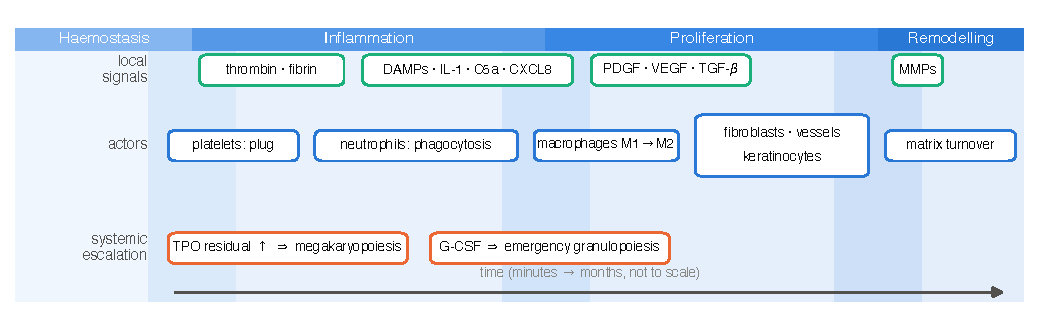
\includegraphics[width=\textwidth]{fig2_timeline}
\caption{The wound-healing response as a phased protocol with three
signal classes. Local signals (aqua) act only on cells carrying the
matching receptor; actors (blue) succeed one another because each
phase's output is the next phase's trigger; systemic escalation
(orange) couples local demand to production of new responders via the
residual loop of Eq.~\ref{eq:integral}. Phase bands are drawn
overlapping, as in vivo: there is no master state machine declaring a
phase boundary --- transitions are population-dynamic. No cell holds a
global plan; timescales indicative.}
\label{fig:timeline}
\end{figure*}

\subsection{Escalation: the residual-signal demand loop}
\label{sec:tpo}

The load-bearing mechanism is the least discussed, and we present it at
three levels: biological mechanism, idealised control law, engineering
principle. \emph{Mechanism}: thrombopoietin (TPO) is secreted
constitutively, chiefly by the liver; circulating platelets and their
marrow progenitors carry the Mpl receptor and clear the hormone from
plasma \citep{kaushansky2005}. When a wound consumes platelets, fewer
receptors remain to clear TPO, the residual rises, and the marrow ramps
megakaryopoiesis until consumption again matches supply; G-CSF runs an
analogous programme for neutrophils under severe demand
\citep{manz2014}. Both systems are richer than any single loop: TPO
clearance is coupled to platelet and megakaryocyte mass and hepatic
output is itself modulated by further physiological cues, so the hormone
is not a purely passive residual detector; and emergency granulopoiesis
is not merely ``G-CSF doing the same'' --- it layers additional
regulation on the G-CSF axis. That richness is exactly why we abstract.

\emph{Control law.} Consider the minimal closed loop: a factory
secreting a constitutive signal; a circulating pool of responders
clearing that signal through receptors, in proportion to their own
availability; a workload consuming responders; production of new
responders driven by the signal, maturing after delay $\tau$; and a
production-relaxation term. With $u$ the responder production rate at
baseline $u_0$, $N$ the responder pool lost at rate $\mu$ and consumed
by workload $w(t)$, $c(t)$ the receptor-mediated clearance of a
constitutive signal flux $p_0$, and $r$ the residual,
\begin{align}
\dot{u}(t) &= \gamma\, r(t) - \beta\,(u(t) - u_0), &
r(t) &= [\,p_0 - c(t)\,]_+,
\label{eq:integral}\\
\dot{N}(t) &= u(t - \tau) - \mu N(t) - w(t)\,N(t), &
c(t) &= \kappa N(t),
\label{eq:pool}
\end{align}
where $[\,x\,]_+ = \max(x, 0)$. Two properties are structural rather
than clipped. First, the signal's production $p_0$ is constitutive ---
not coupled to factory output; the loop closes through the responder
pool, not through the signal, so the causality is depletion $\to$
residual $\to$ production. Second, the residual's non-negativity is
enforced by receptor saturation: clearance is proportional to
responder availability, so depletion --- not instruction --- raises
the residual, and clearance cannot exceed what is circulating. The
factory integrates the residual: a workload depletes $N$, clearance
falls, $r$ rises, and production follows --- without any agent
measuring demand, computing an error, or filing a report. At steady
state the residual settles at exactly the level that sustains the
production the workload requires ($r^{*} > 0$ under sustained demand;
$r \to 0$ only when demand vanishes) --- supply tracks demand in the
sense of matching it, not of zeroing the error. \emph{We are not
claiming that
Eqs.~\ref{eq:integral}--\ref{eq:pool} model wound healing.} They are a
deliberately reduced control motif extracted from one component of the
richer regulation described above --- a model of the abstraction, not
of the biology. The biological claim retained is deliberately minimal:
responder-dependent clearance of a constitutively supplied signal can
encode information about responder availability. Nothing about
physiological equivalence, organ roles or set-points is claimed, and
none is needed for the engineering argument. The decay term is not optional: with $\beta = 0$ the
law is pure integral control and $u$ is monotone non-decreasing, so
after a transient production is frozen at whatever level it reached
--- precisely the fibrotic failure mode of
Section~\ref{sec:pathologies}. Return to homeostasis requires the
antagonist: P3 supplies demand adaptation, P5 supplies reversibility,
and the biology implements both, through clearance kinetics and
explicit antagonists. Coupling fast concentration dynamics to slow
production and maturation makes overshoot and oscillation the expected
transient --- the biology's own oscillations under chronic demand
\citep{manz2014} are the model's stress test and Phase~I's first
theorem. Fig.~\ref{fig:loop} integrates
Eqs.~\ref{eq:integral}--\ref{eq:pool} through a demand pulse: with the
antagonist ($\beta > 0$) the pool recovers and production returns to
baseline; with $\beta = 0$ the same pulse leaves both permanently
elevated --- shown, not merely predicted, for the paper's central law.

\begin{figure}
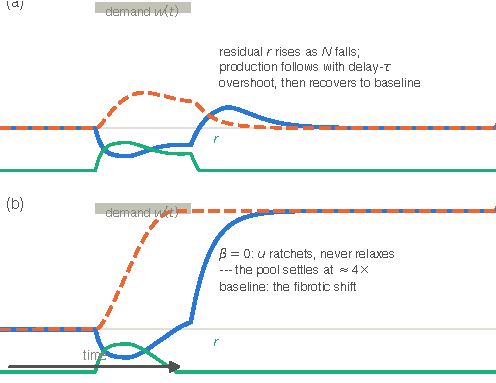
\includegraphics[width=\columnwidth]{fig3_closedloop}
\caption{The closed loop of Eqs.~\ref{eq:integral}--\ref{eq:pool}
through a demand pulse ($\mu = \kappa = p_0 = u_0 = N_0 = 1$,
$\gamma = 1.5$, $\tau = 1.5$; per-capita demand $w = 2$ on $t \in
[5,10)$). (a) With the antagonist ($\beta > 0$): the residual $r$
(aqua) rises as the pool $N$ (blue) falls; production $u$ (orange)
follows with delay-induced overshoot; both return to baseline. (b)
$\beta = 0$: production ratchets and never relaxes; the pool settles
permanently high --- the fibrotic shift. The antagonist term is
mathematically essential, not ornamental.}
\label{fig:loop}
\end{figure}

\emph{Stability.} One simulation is not an analysis, and the loop's
equilibrium and stability structure can be stated already. Under
constant demand $w$, writing $m = \mu + w$ for the total per-capita
loss, Eqs.~\ref{eq:integral}--\ref{eq:pool} admit a
unique positive equilibrium. With the residual inactive
($\kappa u_0/m \ge p_0$), $(u^*, N^*) = (u_0, u_0/m)$ --- at zero
demand $m = \mu$ and this is the baseline $u_0/\mu$; otherwise
\begin{equation}
N^* = \frac{\gamma p_0 + \beta u_0}{\gamma\kappa + \beta m},
\quad\; r^* = p_0 - \kappa N^* > 0, \quad\; u^* = m\, N^* :
\label{eq:eqm}
\end{equation}
sustained demand settles the pool strictly between the fixed-production
ceiling $u_0/m$ (which $N^*$ exceeds exactly when the residual is
active) and the zero-demand baseline $u_0/\mu$ (which it undercuts
whenever $\mu p_0 < \kappa u_0$), with the residual
permanently elevated --- the loop's normal operating point, not a
pathology. Linearising the active branch gives the
characteristic equation
\begin{equation}
(\lambda + \beta)(\lambda + m) + \gamma\kappa\, e^{-\lambda \tau} = 0 .
\label{eq:char}
\end{equation}
At $\tau = 0$ every coefficient is positive and the loop is
unconditionally stable. For $\tau > 0$, putting $\lambda = i\omega$ on
the stability boundary and eliminating the phase $\omega\tau$ yields
$(\gamma\kappa)^2 = (\omega^2 - \beta m)^2 + (\beta + m)^2 \omega^2$,
whose right-hand side is minimised at $\omega = 0$ with value
$(\beta m)^2$: a crossing exists \emph{if and only if}
$\gamma\kappa > \beta(\mu + w)$. Below that threshold the loop is
stable at every delay; above it a Hopf boundary $\tau_H$ appears ---
oscillation is a property of excessive loop gain relative to the
antagonist, which delay exposes and antagonist size prevents. The
inactive branch is linear with roots $\lambda \in \{-\beta, -m\}$,
unconditionally stable. Fig.~\ref{fig:loop}'s parameters must be read
against both branches. At baseline ($w = 0$, $m = \mu$) the loop sits
just above threshold ($\gamma\kappa = 1.5 > \beta m = 1$) at a delay
below $\tau_H$, which is why panel (a) shows damped overshoot; during
the pulse ($w = 2$, $m = 3$) the inequality reverses
($\beta m = 3 > \gamma\kappa = 1.5$), so the loop is below threshold at
every delay --- demand raises the per-capita loss that stabilises the
loop, making it hardest to destabilise exactly when it is working
hardest. Pushing baseline $\tau$
past $\tau_H$ yields the sustained oscillation Phase~II stresses.
Phase~I completes this into a phase diagram over $(\beta \tau,\,
\gamma\kappa/\beta(\mu+w))$ and extends it to finite production
capacity, saturating (Michaelis--Menten) clearance, noisy and delayed
residual measurement, and heterogeneous responders.

\emph{Engineering principle.} In control-theoretic terms,
Eq.~\ref{eq:integral} is a leaky integral controller with anti-windup,
acting on a non-negative, saturating error through a delayed plant
\citep{astrom2008} --- a known object, and we claim no novelty for the
law itself. The novelty is where the error physically resides.
Feedback control of computing systems
already uses integral action \citep{hellerstein2004}: an autoscaler
integrates a \emph{computed} error from a metrics pipeline. The
distinction kept here is where the error lives: measured and integrated
by a controller, or \emph{being} the unconsumed remainder of a consumed
signal, with the medium doing the computing. This law is what no
family in Table~\ref{tab:gap} implements, and it
grounds the programme's deepest hypothesis: \emph{a distributed system
can estimate unmet global demand without explicitly measuring global
demand, because the residual of a consumed signal can itself encode
the error.}

\subsection{Five primitives and one architectural assumption}
\label{sec:principles}

From the protocol and the loop we distil five coordination primitives
(Table~\ref{tab:validation} completes each with its engineering pattern
and falsification test):

\begin{description}
\item[P1 --- Receiver-defined meaning.] The same molecule is a growth
command to one cell and noise to its neighbour; meaning lives in the
receiver's receptors, not in the message.
\item[P2 --- Concentration-as-instruction.] Signals act by local
concentration crossing thresholds, over a medium that diffuses and
decays; instructions are graded and spatially local by physics.
\item[P3 --- Residual-signal-as-demand.] Eq.~\ref{eq:integral}: the
unconsumed remainder of a constitutive signal \emph{is} the demand
estimate.
\item[P4 --- Co-stimulus locality guards.] Effector responses require
a second, local co-signal (damage-associated patterns,
co-stimulation); a solitary systemic signal is not sufficient.
\item[P5 --- Antagonist loops and dissolution.] Every build-up
programme has an antagonist --- the $\beta$ term of
Eq.~\ref{eq:integral} made general --- so structures and responses
have deadlines.
\end{description}

One assumption is conceptually different and we separate it: A1 ---
\emph{cheap items, elastic factories}. Coordinated workers are
expendable and numerous, and production of new workers is elastic and
ignorant --- the marrow does not know where the wound is;
self-replication is an alternative implementation. A1 is an
architectural bet about the substrate, not a coordination primitive.
Whether P1--P5 can coordinate expensive, heterogeneous or
irreplaceable responders, or silently rely on elastic supply, is an
open question the programme tests (Phases~II and V) rather than
assumes.

One disanalogy must be respected from the start. In biology, receptor
identity is fixed by the genome --- a molecule either binds Mpl or does
not; an adversary cannot forge a receptor. In software the receiver's
``receptor'' --- its subscription set --- is dynamic data and can be
spoofed: an adversary emitting a stress key with a chosen identity can
recruit the fleet against itself. Authentication and authorisation are
therefore load-bearing parts of the medium, and P4's co-stimulus
guards --- a second, locally verifiable signal before effector action
--- are the architectural mitigation. Both are attacked in Phase~V.
The mitigation is layered rather than promissory: authenticated
emission and key-scoped receptors fix identity --- the analogue of
genotype-fixed binding; P2's saturation doubles as an innate rate
limit, so flooding has bounded effect; P4 requires a second, locally
verifiable co-signal, so a spoofed systemic signal alone cannot trigger
effector action; and receptor-level anomaly thresholds bound what a
valid-but-malicious insider can recruit --- the sepsis analogue, which
Phase~V attacks deliberately precisely because valid keys defeat
authentication alone.

\begin{table}
\centering
\caption{The validation chain: each primitive at its biological,
abstract and engineering levels, with the result that would falsify
the transfer (Phase~II predictions in parentheses).}
\label{tab:validation}
\footnotesize
\begin{tabular}{@{}lp{16mm}p{16mm}p{16mm}p{17mm}@{}}
\toprule
 & Biology & Abstraction & Engineering & Refuted if \\
\midrule
P1 & thrombin--PAR; TPO--Mpl & receptor set $\Sigma_a$ & handlers & addressed messaging loses nothing \\
P2 & VEGF gradient; quorum & threshold on decaying field & TTL counters & no-decay medium performs as well \\
P3 & TPO residual $\to$ marrow ramp & Eq.~\ref{eq:integral} & autoscaler on residual & no penalty without it (1) \\
P4 & DAMP + co-stimulation & two-signal AND gate & two-factor actuation & no FPR cut (3) \\
P5 & MMPs; IL-10 & decay term $\beta$ & TTL-based GC & $\beta = 0$ still terminates (2) \\
\bottomrule
\end{tabular}
\end{table}

\subsection{Pathologies as safeguards}
\label{sec:pathologies}

The failure modes are as instructive as the successes. Each pathology
illustrates the type of failure that arises when one or more of the
corresponding control functions become inadequate --- a diagnostic
mapping, not a claim of single causation, these diseases being
multicausal: cytokine storm is dominated by P2 runaway
\citep{tisoncik2012}, answered by saturation, rate limits and circuit
breakers; thrombosis is P1/P2 without P4's locality guard, answered by
mandatory co-stimulus checks; autoimmunity is miscalibrated meaning,
answered by burn-in periods in which response rules are learned or
vetoed; fibrosis centrally involves missing P5 ---
Eq.~\ref{eq:integral} with $\beta = 0$, demonstrated in
Fig.~\ref{fig:loop}(b) --- answered by hard dissolution deadlines. Table~\ref{tab:validation}
makes each transfer falsifiable; Phase~V makes the pathologies required
test chapters. A system that does not ship the antagonists of its own
signals has replicated the pathology risk and none of the remedy.

\section{A scientific programme}
\label{sec:programme}

The phases are not a waterfall: the minimal loop is simulated as soon as
it is written (Fig.~\ref{fig:loop}), control analysis feeds revised
models, sandbox anomalies feed back into theorems, and each phase
carries a stated negative-result criterion. The criteria are of two
kinds, and we label each where it is stated: \emph{termination
criteria} --- a result that ends the programme (Phase~I's stability
gate, and Phase~II's prediction~1, both of which kill H1) --- and
\emph{claim-reduction criteria}, where a negative result shrinks the
claim rather than ending it: from ``inevitable'' to ``useful''
(Phase~III), from open fleets to closed fleets (Phase~IV), from
universal to a mapped envelope (Phase~V). The recurring scientific object is delay: fast
concentration coupled to slow production, the
likely source of overshoot and oscillation.

The programme tests three hypotheses that can fail independently.
\emph{H1, mechanistic}: residual consumption is sufficient to estimate
unmet demand --- Eqs.~\ref{eq:integral}--\ref{eq:pool} deliver stable,
reversible demand tracking. \emph{H2, architectural}: the five
primitives together produce robust coordinator-free demand covering
that no subset reproduces. \emph{H3, comparative}: over a defined
operating envelope, the architecture holds a better cost/robustness
frontier than conventional alternatives at equal information and
resource budgets. H1 is tested by Phase~I and prediction~1; H2 by the
Phase~II factorial (predictions 1--3); H3 by Phases~III--IV
(prediction 4). A negative H1 terminates the programme; H2 and H3 can
each fail without taking H1 down, and Table~\ref{tab:decisions} maps
every phase outcome to its response so the falsifiability claims can
be audited rather than admired. The programme also carries two
separable novelties that should not be conflated: a \emph{scientific}
claim --- residual-demand signalling is a stable, discoverable control
mechanism (H1, H2) --- and an \emph{architectural} claim --- it is
competitive on real distributed substrates (H3). H1 can succeed while
H3 fails, and the result would still be interesting: a validated,
biology-derived control law that conventional infrastructure happens
to beat on its own turf is a finding about the biology of control, not
a failure of the science.

\begin{table}
\centering
\caption{Decision table: how phase outcomes map to programme responses.
``Negative'' is the phase's stated criterion firing --- termination
for I and II, claim reduction for III--V; combinations not
shown are revisions --- sandbox anomalies feed back into Phase~I models
by design.}
\label{tab:decisions}
\footnotesize
\begin{tabular}{@{}lp{24mm}p{24mm}@{}}
\toprule
Phase & If negative & If positive \\
\midrule
I & no stable region at realistic $\tau$: \emph{terminate} & stability map secured: proceed \\
II & no P3 penalty: \emph{H1 fails; programme ends as stated} & factorial structure confirmed: H2 stands \\
III & no rediscovery: H1, H2 unaffected; claim narrows from ``inevitable'' to ``useful'' & convergent rediscovery: strongest result \\
IV & substrate cost dominates: H3 fails for open fleets; scope to closed fleets & parity under denial: H3 stands \\
V & envelope too narrow: claims scoped to the mapped envelope & broad envelope: an engineering statement \\
\bottomrule
\end{tabular}
\end{table}

\subsection{Phase I --- Minimal abstraction and controller analysis}

Define a hormonal system $\mathrm{HS} = \langle A, \Sigma, M, R, D
\rangle$: agents $A$; a signal alphabet $\Sigma$; a medium $M$ carrying
concentration fields; threshold-gated response functions $R$; and
degradation/clearance $D$. Two signal classes are distinguished
explicitly, carrying different physics and cost.
\emph{Local fields} serve spatial recruitment,
\begin{align}
\frac{\partial m_s}{\partial t}
  = D_s \nabla^2 m_s - \lambda_s m_s
    + \sum_{a \in A} e_{a,s}(t)\,\delta(\mathbf{x} - \mathbf{x}_a),
\label{eq:medium}
\end{align}
while \emph{well-mixed systemic signals} serve supply loops: their
medium is a circulating pool rather than a spatial field --- TPO is
whole-body --- and their dynamics are the ODEs of
Eqs.~\ref{eq:integral}--\ref{eq:pool}. The phase's first deliverable
is that closed loop itself --- the smallest system containing factory,
pool, workload, clearance and delay --- analysed before the full
$\mathrm{HS}$. Each agent acts on local readings alone:
\begin{align}
u_a(t) = F_a\!\left(\mathbf{1}[m_{s}(\mathbf{x}_a, t) \ge \theta_{a,s}]
\ \text{for}\ s \in \Sigma_a,\ \text{local state}\right).
\label{eq:response}
\end{align}

The committed task class is deadline-constrained demand covering: a set
of sites each requires $r_i$ responders within time $T$ of demand
onset, under churn. The target theorems, with named techniques: (i)
existence and uniqueness of the equilibria of
Eqs.~\ref{eq:integral}--\ref{eq:pool}, their stability, overshoot
bounds and the delay-Hopf boundary of Eq.~\ref{eq:char} --- begun in
Section~\ref{sec:tpo} (unconditional stability at $\tau = 0$; the
delay threshold $\gamma\kappa$ versus $\beta(\mu+w)$) --- completed as
a phase diagram over $(\beta\tau,\, \gamma\kappa/\beta(\mu+w))$ by
linearisation, Routh--Hurwitz and Lyapunov/contraction arguments, and
extended to finite production capacity, saturating
(Michaelis--Menten) clearance, noisy and delayed residual measurement,
and heterogeneous responders; ``realistic''
$\tau$ being anchored in the reference biology: hormone half-lives of
order hours against platelet lifespans of 7--10 days and multi-day
granulopoiesis give $\tau_{\mathrm{production}}/\tau_{\mathrm{signal}}
\sim 10$--$100$, and the theorems must hold across that range; (ii) a
message bound of
$O(n\,k)$ for this class, by potential-function argument, with the
medium's broadcast accounting as $O(1)$ per emission; (iii) termination under antagonist
completeness (every generated
structure has a dissolution rule); and (iv) an impossibility boundary
in the spirit of \citet{fischer1985}: which specifications provably
cannot be met by receiver-only semantics, where coordinators remain
necessary.

The phase's deliverable is a volume, not a tuned point: what fraction
of the anchored parameter box --- $\tau$ spanning the reference ratio
above, $\gamma, \beta, \kappa, \mu, w$ anchored to the ranges the
biology and the Phase~IV substrates motivate --- is asymptotically
stable under the quantitative bounds, and how much of that volume
survives a simultaneous $\pm 20\%$ error in every parameter. A
mechanism that needs four parameters tuned to a few per cent is not a
candidate for robust distributed computing, so the strongest possible
Phase~I result is a large stable volume --- majority, not sliver ---
retained under parameter uncertainty, with Sobol indices naming which
parameters the envelope is most sensitive to and which are safe to
leave unidentified.

The complexity claim is carried by a five-component vector
$(C_{\mathrm{agent}}, C_{\mathrm{medium}}, S_{\mathrm{agent}},
S_{\mathrm{medium}}, L)$: per-agent communication (agent-to-agent
messages), medium communication (emissions, deliveries, bytes,
replication, medium CPU and network work), per-agent state, medium
state, and latency (energy joins $L$ when Phase~IV reaches edge
hardware). A well-mixed broadcast reaches all $n$ nodes: its delivery
cost is $C_{\mathrm{medium}}$, not zero. A coordinator hidden inside
the medium is still a coordinator --- theorem (ii) is honest only if
every component is bounded, and this vector, not a scalar message
count, is the programme's cost statement throughout.

\emph{Termination criterion}: if no parameter region with realistic
production delay $\tau$ --- $\tau_{\mathrm{production}}/
\tau_{\mathrm{signal}} \sim 10$--$100$ --- leaves
Eq.~\ref{eq:char} asymptotically stable with overshoot $\le 50\%$ and
settling within five production delays (the same bounds Phase~V
enforces, so ``stable'' is quantitative: a tolerance, not a vibe), the
load-bearing loop is unsound and the programme ends.

\subsection{Phase II --- Digital wound sandbox}

An executable testbed implementing
Eqs.~\ref{eq:medium}--\ref{eq:response} on discrete topologies, seeded
with three scenario classes translated from biology: \emph{injury}
(node loss or surge), \emph{infection} (sustained load requiring
supply expansion), and \emph{chronic demand} (persistent stress
testing termination). Every run instruments the full
causal chain --- demand $\to$ residual $\to$ production $\to$
population $\to$ recovery. The design instrument is ablation in two
layers: single-principle knockouts, and a factorial design over
P1--P5 with interaction terms, because the primitives' value may be
conditional on each other --- P3$\times$P5 (integration without
antagonist: oversupply and oscillation), P2 without P4 (false
activation), P1$+$P2 without damping (unstable propagation), P4 without P2 sensitivity (failure to
respond). Methodology:
$\ge 30$ seeds per cell, bootstrap 95\% confidence intervals, and
effect sizes preregistered once the noise and adversarial models are
fixed, over a fractional replicate of the $2^5$ design ranked by
first-order Sobol sensitivity indices computed from the Phase~I
linearisation (provisionally $10^5$ simulated node-hours per
scenario class). Beyond the scenario classes, a dedicated
perturbation-and-recovery battery --- step, impulse, ramp, periodic
and stochastic demand; abrupt responder depletion and restoration;
signal delay and loss; heterogeneous receptor thresholds --- measures
rise time, settling time, overshoot, integrated error, oscillation
amplitude, resource excess, communication cost and failure
probability, making the loop a distributed-control experiment whether
or not the biological analogy is credited. P3-removal is not the only
decisive arm: the decisive comparison runs six arms --- full P1--P5;
P3 removed; ordinary measured-error integral feedback granted
identical information; queue/back-pressure control; decentralised
gossip load-balancing; and a central oracle --- answering whether
residual signalling merely works, or confers an identifiable advantage
over conventional feedback at equal information and resources. The
predictions the thesis stands or falls on:
\begin{enumerate}
\item[(H1)] The principal comparison is the outcome vector --- recovery
time, integrated error, overshoot, resource excess, communication
cost, failure probability --- across the six arms at matched
information and budget; the scaling exponent below is one derived
component of it, not the whole test. Without P3, production is fixed
and the pool is capped at the ceiling $u_0/m$, so time-to-resolution
$T = -(1/m)\ln\!\left[(u_0/m - N_T)/(u_0/m - N_0)\right]$ grows
superlinearly in burst size and diverges as the requirement $N_T$
approaches that ceiling, while the full model's demand-tracking
production keeps $T$ near-linear. Phase~I derives the divergence point
and the near-ceiling form; the numeric threshold is preregistered
before the definitive runs.
\item[(H2)] Disabling P5 (antagonists) yields runaway accumulation ---
the fibrosis signature --- in a measurable fraction of chronic-demand
runs.
\item[(H2)] P4's co-stimulus gate strictly reduces false recruitment
($\mathrm{FPR}_{\mathrm{P4}} < \mathrm{FPR}_{\mathrm{no\text{-}P4}}$)
under adversarial signal injection; the effect size is preregistered,
not assumed.
\item[(H3)] Under churn and coordinator-targeted denial, a hormonal fleet
degrades gracefully where a Kubernetes-style orchestrated baseline of
equal steady-state throughput fails outright (A1 alone does not save
it).
\end{enumerate}

\emph{Termination criterion}: if the full model loses to conventional
feedback on the preregistered outcome vector at matched information
and budget --- no penalty for removing P3, no advantage to keeping it
--- the residual loop is not the mechanism the thesis rests on, and H1
fails. A laptop-scale pilot implementation of both phases --- code,
seeds and raw outputs in the repository (\texttt{Jay/phase12}) --- is
reported in Appendix~\ref{app:pilot}; it was run to de-risk the two
termination criteria ahead of the definitive runs, and its findings
are marked where they sharpen the commitments made here.

\subsection{Phase III --- Benchmarks and inverse design}

Hormonal coordination earns its place only against strong
alternatives, in five tiers under identical workloads, information
and resource budgets: a centralised oracle and a near-oracle; a
conventional distributed controller; a state-of-the-art autoscaler
(Kubernetes-style orchestration); the closest field/hormone systems
(gossip membership, stigmergy-style field following); and our own
ablated variants. A comparison against handicapped baselines proves
nothing. The oracle tier is an implementation convenience, not an
architecture: a centralised scheduler granted simulated direct access
to global state at equal compute and message budget --- an upper bound
on what any coordinator could achieve --- while the near-oracle adds
realistic measurement latency; all tiers are run at budgets the phase
polices explicitly. Hand-designing receptor sets will not scale;
the amorphous-computing lesson is to \emph{compile} global shape into
local rules \citep{nagpal2003}, and the synthetic-biology lesson is
that search finds rule sets analysis cannot \citep{basu2005, you2004}.
The programme therefore includes evolutionary search over an extended
genotype --- $(\Sigma, R, \theta)$ plus medium parameters $(\lambda, D,
\gamma, \beta)$ and affinity/antagonist relationships --- scored
against two target specifications (deadline covering; graceful
degradation under churn) under a fixed compute budget (provisionally
$10^6$ evaluations per specification). The joint space is not searched
blind: a pilot --- fixed topology, two or three loci free at a time
--- validates the fitness landscape before the extended genotype is
released. Search output is
not trusted for fitness alone: high-fitness solutions are audited
against Phase~I's preconditions and inspected for which primitives
they use.

The audit carries the scientific payload and the programme's central
evolutionary hypothesis: \emph{deprived of global state but required
to solve variable-demand resource allocation robustly, optimisation
independently evolves residual-demand signalling.} The test is run on
a ladder of progressively stronger global-information restrictions,
so the motif's emergence --- if it emerges --- can be attributed to
the restriction and not the fitness function. The search is also
blind, with the blindness frozen in advance: the genotype, the fitness
function, the information budget, the criteria for judging a loop
P3-like, and the classification procedure are all fixed and dated
before the first run of the released genotype; the genotype carries no
signal semantics, the fitness function
never names primitives, and evolved architectures are classified only
after the runs complete --- de-identified, with condition labels
unblinded after every solution is classified --- so rediscovery is
convergent evidence, not scaffolding. The joint space is of order
$10^2$ dimensions (eight signal loci with emission, response and
threshold genes each, four medium parameters, an $8 \times 8$
affinity/antagonist matrix), which is why the pilot measures the
landscape's correlation length before the full release. Does search
rediscover the biological motifs --- co-stimulus gating, antagonist
pairing, constitutive-and-consumed signals --- without being told to?
If audited solutions
converge on P3-like loops across specifications, the primitives are a
general control architecture rather than biology trivia --- evidence
of convergent discovery by biological evolution and computational
optimisation, and the programme's most impressive possible result.

\emph{Claim-reduction criterion}: if audited solutions that meet
specification never contain residual-demand loops, P3 is not a
discoverable general mechanism --- the claim narrows from ``a general
control architecture'' to ``a hand-designed one''; H1 and H2 are
unaffected.

\subsection{Phase IV --- Substrate engineering}

Deployment needs a medium with the physics of Eq.~\ref{eq:medium},
which present-day infrastructure approximates: publish--subscribe with
per-key time-to-live aggregation windows provides diffusion-and-decay
counters; sidecars provide the receptor abstraction over legacy
services; conflict-free replicated data types \citep{shapiro2011} give
idempotent resumption when responders die mid-task. Before either
pilot, a medium audit connects Eq.~\ref{eq:medium} to the discrete
substrate: emulation on a grid testbed measures the approximation
error of TTL aggregation against the continuous field, and the pilots
proceed only if that error is bounded --- Phase~I's guarantees must
survive the discretisation they are deployed on.

The medium's own failure modes are part of the architecture, not an
afterthought. Under partition, concentration fields decay in place,
and staleness is self-announcing: a decaying signal reads as
\emph{less} demand, so a partitioned region under-responds rather
than mis-responds, with local baseline capability carrying the
interval. Concentration semantics also relax delivery requirements:
aggregation is commutative and idempotent, so at-least-once delivery
with per-key time-to-live is sufficient, message ordering is
irrelevant, and exactly-once semantics --- so expensive in messaging
systems --- are simply not needed. Sustained medium loss remains
fatal to escalation (the residual cannot be transported), which is
why medium availability and partition behaviour are axes of the
Phase~V boundary rather than footnotes.

Two pilots, each
with success criteria stated against existing practice: (a)
microservice incident self-management: a stressed service emits a
stress key, co-stimulus-gated responders drain queues and shed load,
and an autoscaler keyed on the \emph{residual} of a constitutive
heartbeat replaces metrics pipelines --- the criterion is parity with
a Kubernetes horizontal autoscaler and an event-driven autoscaler in
the KEDA style on benign step loads, responding no
slower than one metrics interval, under identical replica counts,
network allocation and response capacity for both sides, while
surviving coordinator-plane denial that kills both and riding
through an injected 30-second medium partition with no erroneous
action (fields decay in place, behaviour falls back to local
baseline capability, recovery proceeds without thrash);
(b) edge/swarm task allocation, an AHS-scale problem
\citep{brinkschulte2008} extended with supply dynamics --- the
criterion is throughput within 10\% of a centralised assigner at
10$\times$ the fleet size, at bounded $C_{\mathrm{medium}}$, under
the same medium-partition ride-through criterion.

\emph{Claim-reduction criterion}: if the medium's substrate cost
dominates the
coordination saved on realistic fleets, the architecture is a renaming
of the coordinator --- H3 fails for open fleets, and the claim is
scoped to closed fleets rather than abandoned.

\subsection{Phase V --- Failure theory and the operating boundary}

Section~\ref{sec:pathologies}'s four pathologies become required test
chapters, each with quantitative damping bounds rather than happy-path
demonstrations: signal spoofing (the sepsis
analogue --- an adversary injecting stress keys to exhaust the
factory; mitigated by medium authentication and P4, attacked
directly), storm cascades, miscalibration after topology change, and
fibrotic accumulation. And the question the existence proof cannot
answer must be answered here: \emph{where is the operating boundary?}
The programme maps degradation against demand amplitude, spatial
extent, latency, noise and responder depletion --- severe trauma
overwhelms even biology --- and delivers the boundary as an
operating-envelope map,
\begin{align}
F(&\text{demand}, \tau, \text{noise}, \text{churn}, \text{capacity},
\nonumber\\
&\quad \text{attack rate}, \text{medium availability}) \nonumber\\
&\to \{\text{stable}, \text{underdamped}, \text{oscillatory},
\text{runaway}, \text{collapse}\},
\label{eq:envelope}
\end{align}
summarised as phase diagrams ---
$\tau_{\mathrm{production}}/\tau_{\mathrm{signal}}$ against
peak demand over baseline capacity, and $\beta\tau$ against
normalised loop gain $\gamma\kappa/\beta(\mu+w)$ from
Eq.~\ref{eq:char} --- turning
``severe trauma overwhelms even biology'' into a quantitative
operating envelope. Provisional targets: post-step
overshoot $\le 50\%$ (a bound matched to typical autoscaler error
budgets, and revisited against Phase~II data), recovery to within
10\% of baseline within five
production delays, zero runaway accumulations in $10^4$
chronic-demand node-hours --- aligned with conventional autoscaling
SLOs and error budgets, to be tightened after Phase~II. The headline
deliverable is a region statement, not a point claim: the envelope map
names where hormonal coordination \emph{dominates} (high churn and
coordinator-targeted denial, where the medium's cost is amortised and
the coordinator is the attackable part), where it is merely
\emph{comparable} (benign steady loads, where conventional feedback is
good enough), and where it \emph{fails} (sustained partition and
extreme latency, where the medium itself is the bottleneck). Only then
does
``coordination without a
coordinator'' become an engineering statement with a known domain.

\emph{Claim-reduction criterion}: an operating envelope too narrow to
cover
operationally relevant workloads scopes the architectural claim to the
mapped envelope --- H3 survives inside it and is not asserted outside
it.

\subsection{Feasibility and resourcing}
\label{sec:feasibility}

The programme is sized as a small-team effort of roughly three years,
and its budgets are derived rather than asserted. Phase~I is analyst
work plus laptop-scale numerics ($\sim 10^3$ core-hours). Phase~II's
$10^5$ node-hours follow from the design: $\ge 30$ seeds per cell
resolves standardised effects $d \gtrsim 0.7$ at 95\% confidence with
bootstrap intervals, and the budget covers the fractional factorial,
the perturbation battery and the six-arm comparison across three
topologies. Phase~III's $10^6$ evaluations run in weeks on a 64-core
node once the pilot has validated the fitness landscape; Phase~IV
requires two engineers and existing cluster hardware; Phase~V is
analyst and red-team time. The compute figures are initial budgets,
and compute is not the binding constraint: Phase~III's expensive parts
are design, implementation, artefact recognition and validation ---
building the simulator, the blinding protocol and the classifier,
redesigning fitness after the pilot, auditing evolved solutions for
hidden global state --- which are engineer-months, not core-hours.
Every budget is provisional, gated by the
preceding phase's pilot, and allocated by the computed Sobol ranking
--- so a funding panel can audit each number back to a design choice
rather than a guess.

\section{Discussion}
\label{sec:discussion}

Three clarifications keep the thesis honest. First, the complexity
claim is a vector, not a scalar: the agent-side components of
$(C_{\mathrm{agent}}, C_{\mathrm{medium}}, S_{\mathrm{agent}},
S_{\mathrm{medium}}, L)$ fall to $O(n\,k)$ conditional on
a medium providing broadcast, locality and decay, while what that
medium spends is a real cost
paid in Phase~IV; the medium is the load-bearing wall, and without
decay, concentration semantics degenerate and with them P2 and P3. Second, the class of reachable
behaviours is restricted to what threshold logic on fields can
express; Phase~I's impossibility results are expected to show that
some specifications (strict global invariants, exact sequencing)
genuinely require coordinators. The claim is not that coordinators are
never needed; it is that a large, operationally important class ---
incident response, load balancing, supply tracking,
cleanup --- does not need them, and pays less for not having them.
Third, biology keeps centralised \emph{production} (A1); the argument
is against centralised \emph{deciding} --- the marrow does not know
where the wound is, and does not need to.

The comparison to autonomic computing
\citep{kephart2003} is generational: autonomic systems report to a
control loop; a hormonal system embeds the control loop in the
medium and lets the residual do the reporting. If the programme's
predictions hold, the practical outcome is systems whose coordination
cost does not compound with scale --- where, within the mapped
operating envelope, the thousandth node is as
cheap to coordinate as the tenth, because it joins a medium rather
than a meeting.

\section{Conclusions}
\label{sec:conclusions}

We have posed coordinator-free coordination as a precise question,
shown that wound healing answers it once in nature over a substantial
operating envelope, distilled that answer into five testable
coordination primitives plus one architectural assumption,
derived the central control law's equilibria and delay-stability
threshold and demonstrated its fibrotic failure mode in
simulation (Fig.~\ref{fig:loop}), located the
gap in the sixteen families surveyed (the residual-signal demand loop
above all), and specified a five-phase programme with falsifiable
predictions, stated criteria per phase --- terminal for the core
mechanism, claim-reducing elsewhere --- and a decision table ---
testing
three separable hypotheses: mechanistic (H1), architectural (H2) and
comparative (H3), whose two novelties are separable: the science of
the residual loop can stand even where its engineering case does not.
The programme's terminal output is a dominance map --- where hormonal
coordination wins, where it ties, and where it should not be used.
The
question the programme answers is the one the introduction asked; the
standard of success is the one the reference system already meets:
many items, each knowing the bare minimum, doing excellent work
together.

\section*{Acknowledgements}

Developed within the BIODISC (Biology Discovery and Intelligence
System) environment, an independent research laboratory. Analysis and
drafting were assisted by AI research tooling (Claude, Anthropic);
the programme, its judgements and its claims are the author's.

\appendix

\section{Search methodology for the gap analysis}
\label{app:search}

The gap analysis of Table~\ref{tab:gap} was run as a falsification
directed search: the goal was not to assemble supporting citations but
to find an architecture that implements P3 natively and thereby
falsify the claimed gap before publication.

\emph{Protocol.} Sources: Google Scholar, ACM Digital Library, IEEE
Xplore, arXiv (cs.MA, cs.DC, eess.SY) and PubMed for the
biology-side precedents. Query families: hormone/endocrine regulation
for multi-robot and distributed coordination; residual or unconsumed
signal as demand estimate; antithetic and sequestration integral
feedback; pheromone, digital pheromone and stigmergy at scale;
back-pressure and congestion-driven capacity scaling; event-driven and
metric-pipelined autoscaling; amorphous and homeostatic computing.
Each family's literature was then snowballed through its own
taxonomies and reviews. The original survey was assembled 2026-07 and
the currency re-sweep of post-2016 threads was run 2026-08-15.

\emph{Inclusion and scoring.} A candidate enters the table if it
claims distributed coordination or resource allocation through signal
fields or a chemical metaphor. The P1--P5 and A1 definitions
(Section~\ref{sec:principles}) were fixed before any family was
scored. The rubric: P1 is native when receiver-side selection is
load-bearing, partial when addressing dominates; P2 is native when
graded, decaying concentration is load-bearing, partial when signals
are binary; P3 is native only when a constitutively produced quantity
is cleared in proportion to available responding capacity and its
residual drives capacity creation --- partial when a measured backlog
or computed error approximates the residual; P4 native when two-signal
gating is required for effector action; P5 native when antagonist
dissolution terminates responses.

\emph{Dispositions of the post-2016 threads.} Antithetic
sequestration control has been realised experimentally since
\citet{briat2016}, in living and cell-free systems \citep{aoki2019},
but remains a single-volume controller: no broadcast medium, no
receiver-defined semantics --- row unchanged. Pheromone stigmergy has
been tested to its limits at high swarm density \citep{hunt2019};
the repertoire is spatial recruitment, with no constitutive-consumed
residual --- row unchanged. Event-driven autoscaling in the KEDA style
scales on queue depth and event backlog --- a genuine residual, but
one measured and integrated by a controller through a metrics
pipeline; its canonical sources are project documentation and vendor
literature rather than peer-reviewed evaluations, which we note as a
finding about the thread, and it is scored under congestion/back-pressure ---
row unchanged. Successors of the artificial-endocrine family keep the
hormone as a node-computed score; no post-2016 system found couples a
constitutive broadcast to consumption-proportional clearance driving
capacity creation.

\emph{Commitments.} The frozen definitions, the query list, the dates
and this rubric are preregistered with the Phase~I--II registration.
Before submission, an independent second scorer rescores every family
against the same frozen definitions; disagreements are resolved by
documented discussion, and both scorings will be published with the
paper.

\section{Phases I--II pilot: implementation and first results}
\label{app:pilot}

This appendix reports a pilot execution of the Phase~I and Phase~II
commitments (Sections~4.1--4.2), run on 2026-08-16 to de-risk the
programme's two termination criteria before the definitive runs.  The
pilot implements the closed loop of Eqs.~\ref{eq:integral}--\ref{eq:pool}
as a delay differential equation integrated by Euler steps with a
ring-buffer maturation history, and the sandbox of
Eqs.~\ref{eq:medium}--\ref{eq:response} on a $24\times24$ torus with
positivity-preserving donor-cell advection; P1--P5 are compile-time
toggles and the six arms are production/redistribution policies on the
same plant.  Every draw is through a seeded \texttt{numpy} generator;
code, seeds and raw outputs are in the repository
(\texttt{Jay/phase12}: \texttt{jay\_core.py}, \texttt{sandbox.py},
\texttt{run\_phase1.py}, \texttt{run\_phase2.py},
\texttt{phase1\_results.json}, \texttt{phase2\_results.json}).  The
entire pilot --- all sweeps, both phases --- runs in under three
minutes on one laptop.  It is not the definitive study: 30 seeds per
sandbox cell, one grid resolution, and no preregistered effect sizes;
its numbers are descriptive.  Its purpose is to find, early and
cheaply, the places where the programme's stated commitments meet an
unfriendly numerical reality; five such findings are collected in
Section~\ref{app:pilot-changes}.

\subsection{Phase I pilot: the minimal loop}
\label{app:pilot-1}

\emph{Setup.}  The normalisation $\kappa = p_0 = 1$, $u_0 = \mu$
makes the no-demand baseline $N = 1$ with zero residual, generalising
Fig.~\ref{fig:loop}'s.  The anchored box of Section~4.1 is sampled
log-uniformly in its five free dimensions: $\mu \in [10^{-2},10^{-1}]$
(responder lifespans), $\beta \in [10^{-2},0.3]$ (production
relaxation), $\tau \in [10,100]$ (the reference ratio
$\tau_{\rm production}/\tau_{\rm signal}$), loop gain
$y = \gamma\kappa/\beta(\mu+w) \in [0.5,10]$ (the ordinate of the
Section~4.1 phase diagram, so $\gamma$ is fixed by the drawn $y$), and
demand $w/\mu \in [1,10]$.  A box point \emph{passes the quantitative
gate} if the active branch is asymptotically stable under
Eq.~\ref{eq:char} \emph{and} the simulated step response overshoots
the target by $\le 50\%$ \emph{and} settles within the $\pm5\%$ band
in at most five production delays --- the same bounds Phase~V
enforces.

\emph{Equilibria.}  Across 400 box points, the simulated final state
matches Eq.~\ref{eq:eqm} to 0.55\% (95th percentile) wherever the
response has converged ($\tau < 0.5\,\tau_H$); the error tail (6.7\%
at the 95th percentile over all stable points) sits entirely at
$\tau/\tau_H \in [0.5,1)$, where damped ringing outlasts the $12\tau$
integration window --- slow convergence near the boundary, not
integrator bias.

\emph{Phase diagram.}  Fig.~\ref{fig:pilot1}(a) plots the closed-form
Hopf boundary $\tau_H$ of Eq.~\ref{eq:char} in the $(\beta\tau, y)$
plane at three values of $m/\beta$, with the Monte-Carlo box overlaid
in the same coordinates.  Simulated oscillation onset coincides with
the analytic boundary: at the Fig.~\ref{fig:loop} slice, the
last-quarter amplitude is $\le 0.002$ at $0.5\,\tau_H$, jumps
$\times4$ across $\tau_H$ (0.0125 at $0.8\,\tau_H$ to 0.047 at
$\tau_H$ at $y=1.5$) and keeps growing to 0.083 at $2\,\tau_H$; the
same stair-step appears at $y = 3$ and $y = 6$.

\begin{figure*}
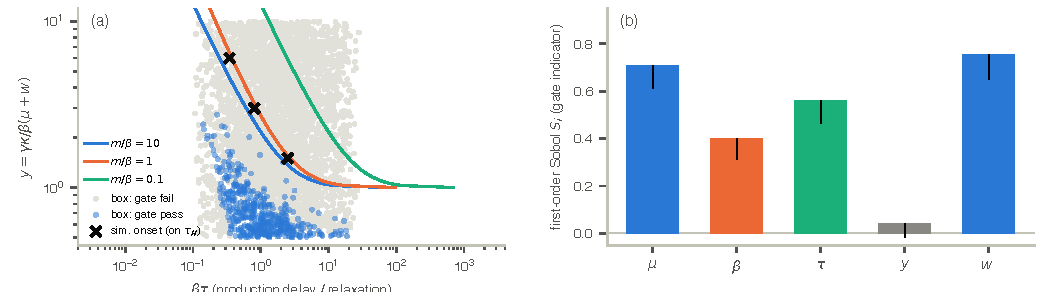
\includegraphics[width=\textwidth]{figA1_phase1}
\caption{Phase~I pilot.  (a) The delay-Hopf boundary of
Eq.~\ref{eq:char} in the $(\beta\tau,\, y)$ plane of Section~4.1 at
three $m/\beta$ contours (lines, left to right: $m/\beta = 10$, 1,
0.1); the anchored parameter box overlaid as pass (blue) / fail
(grey) against the quantitative gate; $\times$ marks simulated
oscillation onset, placed at $\tau = \tau_H$.  (b) First-order Sobol
indices of the gate indicator (covariance estimator, Saltelli
$A/B$ matrices, $N=1024$, bootstrap 95\% confidence intervals): the
envelope is set by timescales and demand ($\mu$, $w$, $\tau$,
$\beta$), not by loop gain $y$.}
\label{fig:pilot1}
\end{figure*}

\emph{Gate volume --- the honest number.}  Over $2^{12}$ box points:
45.9\% are asymptotically stable, 36.3\% meet the overshoot bound,
and 11.5\% settle within five production delays --- the gate volume
is 11.5\%, and \emph{settling is the binding criterion} (median
settling among passers: $4.17\,\tau$; median overshoot: 10\%).  Under
eight simultaneous $\pm20\%$ perturbations of all five dimensions,
50.3\% of passing points survive every draw (5.8\% of the box
unconditionally).  Against Section~4.1's hope of ``majority, not
sliver'', the pilot finds a sliver --- and Section~\ref%
{app:pilot-changes} records the two candidate responses (denominate
the settling budget in the loop's slowest timescale, or report the
volume honestly).  The termination criterion itself is \emph{not}
triggered: a realistic-delay region passing all three bounds with
majority robustness exists.

\emph{Sensitivity.}  First-order Sobol indices of the gate indicator
(Fig.~\ref{fig:pilot1}b): $w$ 0.75 [0.65, 0.86], $\mu$ 0.71 [0.61,
0.81], $\tau$ 0.56 [0.47, 0.68], $\beta$ 0.40 [0.31, 0.50], and loop
gain $y$ 0.04 [$-0.02$, 0.11] (bootstrap 95\% CIs).  The inversion is
the useful result: which parameters must be identified carefully are
the timescales and the demand; the loop gain that the stability
analysis centres on is, within the anchored box, nearly free ---
exactly the parameter the biology leaves unpinned across an order of
magnitude.  The indices sum to well above one's expectation for an
additive decomposition (2.5), i.e.\ the gate fails through
interacting parameter combinations, consistent with settling being
governed by the slowest of $\{\tau, \beta^{-1}, m^{-1}\}$.

\emph{Extensions.}  Table~\ref{tab:ext} gives the gate volume under
the four named extensions.  Finite capacity and Michaelis--Menten
clearance \emph{help} (both self-limit overshoot); heterogeneity
costs a third of the volume; and the delayed+noisy measurement arm
collapses it --- decomposed, the collapse is entirely measurement
\emph{latency}, not measurement \emph{noise}: with $\sigma = 0.1$
sampled-and-held jitter and no delay the volume is unchanged (the
integral loop averages the jitter), while a pure residual-measurement
delay of $0.1\,\tau$, $0.25\,\tau$, $0.5\,\tau$ gives 0.091, 0.048,
0.015.  The minimal model's assumption that the medium relaxes on the
signal timescale is load-bearing: the factory must see the residual
fast relative to its own production delay, or the settling budget is
spent before the loop begins.

\begin{table}
\centering
\caption{Phase~I gate volume under the four named extensions
($n = 2048$ box points each; baseline re-drawn per arm).}
\label{tab:ext}
\begin{tabular}{lc}
\toprule
arm & gate volume \\
\midrule
baseline & 0.123 \\
finite capacity ($u \le 4u_0$) & 0.140 \\
Michaelis--Menten clearance & 0.146 \\
heterogeneous responders & 0.085 \\
measurement noise only ($\sigma = 0.1$) & 0.123 \\
residual delay $0.1\,\tau$ only & 0.091 \\
residual delay $0.25\,\tau$ only & 0.048 \\
delayed$+$noisy residual ($0.5\,\tau$, $\sigma=0.1$) & 0.015 \\
\bottomrule
\end{tabular}
\end{table}

\emph{The no-P3 divergence (closed-loop face of H1).}  With demand on
throughout and a burst removing 70\% of the pool ($N_0 = 0.3$ under a
fixed-production ceiling $u_0/m = 0.5$), Table~\ref{tab:nop3} compares
the simulated time to reach $N_T = (1-\varepsilon)\,u_0/m$ against
the closed form $T = -(1/m)\ln[(u_0/m - N_T)/(u_0/m - N_0)]$.  The
fixed-production arm matches the closed form to $\le 0.1\%$ at every
$\varepsilon$ and diverges logarithmically as $\varepsilon
\rightarrow 0$, while the demand-tracking loop ($y = 0.6$,
delay-unconditionally stable) saturates at $\approx 1.1\,\tau$: at
$\varepsilon = 1.6\times10^{-3}$ the contrast is $2.6\times$ and
growing without bound.  Near the ceiling the two arms agree, as they
must --- the loop has not yet had time to matter.

\begin{table}
\centering
\caption{No-P3 divergence: time to reach $N_T = (1-\varepsilon)\,
u_0/m$ from $N_0 = 0.3$ ($\mu = w = 0.05$, $m = 0.1$, ceiling
$u_0/m = 0.5$; tracking loop $y = 0.6$, $\tau = 20$).  ``Theory'' is
the closed form of H1 for the fixed arm.}
\label{tab:nop3}
\begin{tabular}{lccc}
\toprule
$\varepsilon$ & $T_{\rm fixed}$ (sim) & $T_{\rm fixed}$ (theory) &
$T_{\rm tracking}$ (sim) \\
\midrule
0.355 & 1.20 & 1.20 & 1.20 \\
0.092 & 14.72 & 14.73 & 14.72 \\
0.024 & 28.24 & 28.25 & 21.22 \\
0.0061 & 41.74 & 41.78 & 21.62 \\
0.0016 & 55.26 & 55.31 & 21.72 \\
\bottomrule
\end{tabular}
\end{table}

\subsection{Phase II pilot: the digital wound sandbox}
\label{app:pilot-2}

\emph{Setup.}  Three sites of demand on a $24\times24$ torus;
responders migrate up the sensed gradient above threshold
($\chi$-limited, donor-cell advection) and are expended by serving;
the systemic loop of Eqs.~\ref{eq:integral}--\ref{eq:pool} couples a
factory (delay $\tau = 20$, antagonist $\beta$) to the grid-total
pool through the residual $r = [1 - \kappa N]^+$.  Scenario classes:
\emph{injury} (one-shot demand), \emph{infection} (demand refills at
constant rate), \emph{chronic} (refilling demand that clears at
$t = 6\tau$).  Routine housekeeping traffic --- diffusive distractor
pulses that receiver-correct responders must ignore --- runs
throughout (P1's payload).  30 seeds per cell; every metric below is
over seeds; the deadline is $8\tau$.

\emph{Factorial knockout.}  Table~\ref{tab:factorial} regresses the
failure indicator on the five toggles plus the three named
interactions ($2^5$ cells, infection scenario).  P3 dominates:
knocking out the residual loop costs $0.763$ [$-0.808$, $-0.708$] in
failure probability --- every P3-less cell fails outright under
infection, exactly the no-P3 ceiling of H1.  P2 and P4 knockouts cost
$0.075$ and $0.083$.  The P3$\times$P5 interaction is the largest
conditional effect ($-0.175$): the antagonist's dissolution pays only
when there is a loop to terminate --- with P3 present, adding P5 cuts
failure from 0.24 to 0.07 averaged over the stratum; with P3 absent
it is irrelevant.  (The P5 main effect is unidentified rather than
zero: all sixteen P3-less cells fail at exactly 1.0, so the saturated
stratum has no variance and the effect loads entirely on the
interaction.)  The P2$\times$P4 term ($-0.058$, CI marginally
excluding zero) points the same way as the design intent: the
co-signal guard substitutes for some of the selectivity that
threshold-free responders lose.  P1 is failure-neutral at these
distractor loads (its cost appears as misallocated holding, not
failed episodes) --- an honest null.

Two further readings of the cell means matter for the definitive
design.  First, in the \emph{benign} infection scenario the P3-only
cell fails least of all (0.00 failure, 0.059 unmet, versus 0.10 /
0.077 for the full stack): the guard and the antagonist each trade a
little throughput for safety that this scenario does not bill ---
their value appears precisely where H2 and H2b bill it.  Second, the
P4 knockout \emph{raises} failure here (0.00 $\to$ 0.33 in the
P3-only stratum) because serving gated by the co-signal is slower
\emph{and} because without the guard, responders burn at stale halos
left by cleared sites --- friendly fire, not adversarial fire.  The
primitives are throughput costs and robustness gains, which is the
paper's argument for reporting the full outcome vector rather than
latency alone.

\begin{table}
\centering
\caption{Factorial knockout regression on the infection scenario
($2^5$ cells $\times$ 30 seeds; toggle coded 1 = knocked out; OLS on
cell means, bootstrap-over-seeds 95\% CIs).}
\label{tab:factorial}
\begin{tabular}{lcc}
\toprule
term & failure & unmet \\
\midrule
intercept & $+0.937\;[0.914, 0.960]$ & $+0.190\;[0.180, 0.199]$ \\
P1 & $-0.008\;[-0.038, 0.025]$ & $-0.006\;[-0.014, 0.002]$ \\
P2 & $+0.075\;[0.033, 0.119]$ & $+0.005\;[-0.004, 0.014]$ \\
P3 & $-0.763\;[-0.808, -0.708]$ & $-0.109\;[-0.115, -0.102]$ \\
P4 & $+0.083\;[0.050, 0.119]$ & $-0.011\;[-0.018, -0.004]$ \\
P5 & (unidentified; text) & $+0.064\;[0.053, 0.073]$ \\
P3$\times$P5 & $-0.175\;[-0.236, -0.112]$ & $-0.070\;[-0.080, -0.059]$ \\
P2$\times$P4 & $-0.058\;[-0.117, 0.004]$ & $+0.000\;[-0.010, 0.010]$ \\
P1$\times$P2 & $+0.008\;[-0.052, 0.069]$ & $+0.005\;[-0.005, 0.015]$ \\
\bottomrule
\end{tabular}
\end{table}

\emph{Six arms at matched information.}  Table~\ref{tab:arms} reports
the decisive comparison across the three scenarios, with the
medium-side cost vector.  The honest ordering on latency: the oracle
resolves fastest ($0.31\,\tau$, reading global state); queue/back-
pressure and gossip next ($0.9\,\tau$, routing directly on per-cell
load); the two residual-driven arms at $3.5$--$4.8\,\tau$; fixed
production fails outright wherever demand refills.  The
\emph{measured-error} arm --- an ordinary integral controller granted
site reports --- tracks the physical residual almost exactly (within
2\% on resolve time and unmet, infection) at $1.5$ messages per unit
time: the medium computes the same integral for free, and that
equivalence, not superiority, is the correct reading of P3 at this
scale.  The hormonal arm's case is carried by the other axes of the
vector: zero agent-side messages, graceful degradation under
coordinator denial (below), and no second infrastructure to keep
alive.  The sandbox's medium bill is real and must not be hidden: the
field arms pay $\sim\!10^5$ cell-deliveries per unit time against
gossip's $3.8\times10^3$ messages --- the price of a physics nobody
has to route.

\begin{table*}
\centering
\caption{The six Phase~II arms at matched information and budget
(30 seeds; time in production delays $\tau$; deadline $8\tau$).
Resolve = median time to clear demand (censored at run end).  Cost
components per unit simulated time on the $24\times24$ grid
(infection scenario; an emission bills $G^2 = 576$ cell-deliveries;
all arms additionally hold $3G^2$ words of agent state).}
\label{tab:arms}
\begin{tabular}{l ccc cccc}
\toprule
& \multicolumn{3}{c}{failure / resolve ($\tau$)} &
\multicolumn{4}{c}{cost per unit time} \\
\cmidrule(lr){2-4}\cmidrule(lr){5-8}
arm & injury & infection & chronic &
emissions & deliveries ($10^3$) & messages & medium state (words) \\
\midrule
hormonal (P1--P5) & 0.00 / 3.6 & 0.10 / 4.8 & 0.03 / 4.8 &
191 & 110 & 0 & 2304 \\
fixed (no P3) & 0.73 / $>8$ & 1.00 / $>8$ & 1.00 / $>8$ &
191 & 110 & 0 & 2304 \\
measured-error & 0.00 / 3.5 & 0.10 / 4.7 & 0.03 / 4.7 &
191 & 110 & 1.5 & 2304 \\
back-pressure & 0.00 / 0.9 & 0.00 / 0.9 & 0.00 / 0.9 &
1.5 & 0.9 & 0 & --- \\
gossip & 0.00 / 0.9 & 0.00 / 0.9 & 0.00 / 0.9 &
--- & --- & 3848 & --- \\
oracle & 0.00 / 0.3 & 0.00 / 0.3 & 0.00 / 0.3 &
--- & --- & 0 & --- $^{\dagger}$ \\
\bottomrule
\end{tabular}

$^{\dagger}$the oracle instead reads global state ($G^2$ words per
read, continuously): a coordinator hidden in the instrumentation, by
design the upper bound.
\end{table*}

\emph{H1, sandbox face (Fig.~\ref{fig:pilot2}a).}  Sweeping demand
mass $D$ from 2 to 12 baseline units (injury): the hormonal arm's
median resolve time grows near-linearly ($26 \to 148$, slope
$\approx 12$ per unit $D$) with production scaling $u_{\rm peak}/u_0
= 3.5$--$3.8$; the fixed arm cannot scale ($u_{\rm peak}/u_0 = 1.0$
throughout), fails 33\% at $D=4$ and 100\% from $D = 8$.  The
tracking arm's own failures at $D \ge 10$ (17\%, 40\%) are honest:
they are serving-and-migration limits of the grid, not loop limits
--- production was still scaling when the deadline expired.

\emph{H2, fibrosis (Fig.~\ref{fig:pilot2}b, bars).}  Chronic demand
clearing at $t = 6\tau$: with P5 the pool stands down to $1.03\times$
baseline and production to $1.00\times$; without P5 the pool
ratchets to $3.07\times$ and production to $3.10\times$ and stays
there --- Fig.~\ref{fig:loop}(b)'s fibrotic shift, reproduced with
spatial routing in the loop, in a measurable fraction of runs
(failure 13\% versus 3\%).

\emph{H2b, adversarial recruitment (Fig.~\ref{fig:pilot2}b, lines).}
Sweeping false-signal injection rate $\nu = 0 \to 0.2$: with the P4
co-signal gate, false burn is \emph{zero} at every $\nu$; without it,
burn rises from 12 (at $\nu = 0$ --- friendly fire at stale halos) to
78 pool mass at $\nu = 0.2$.  Misallocated holding is similar in
both arms ($\sim$5--11): P4 gates \emph{expenditure}, not attention
--- the guard's FPR claim holds, and its cost shows up as the
throughput tax of Table~\ref{tab:factorial}.

\emph{H3, coordinator denial and churn.}  The oracle arm under two
outages of its coordinator channel ($(0,30)$ and $(50,90)$, 35\% of
the run): unmet demand rises $6.5\times$ over the clean oracle (0.104
versus 0.016) --- to \emph{worse than the hormonal arm} (0.077),
which has no coordinator to deny.  The hormonal arm under churn
(random removal of 10--50\% of off-site responders every $\tau$) does
not degrade: failure 0.10 $\to$ 0.03, unmet 0.077 $\to$ 0.073 ---
turnover prunes the wandering pool, keeps the residual honest, and
sustained delivery continues; the loop is robust to, even mildly
aided by, the constant turnover its biological reference runs
natively.

\begin{figure*}
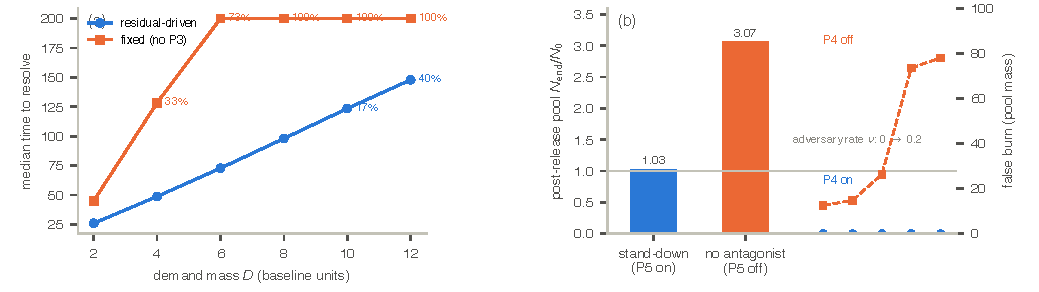
\includegraphics[width=\textwidth]{figA2_phase2}
\caption{Phase~II pilot.  (a) H1: median time to resolve versus
demand mass $D$ (injury scenario; deadline $8\tau$): the residual-
driven arm scales production ($u_{\rm peak}/u_0 = 3.5$--$3.8$) and
resolves near-linearly, with graceful degradation at $D \ge 10$;
fixed production cannot scale and fails outright (percentages:
failure rate).  (b) H2/H2b: bars --- post-release pool $N_{\rm
end}/N_0$ in the chronic scenario with the antagonist (P5) on and
off, the fibrotic shift; lines --- false burn (expended pool mass)
versus adversary rate $\nu$ with the P4 co-signal gate on and off.}
\label{fig:pilot2}
\end{figure*}

\subsection{What the pilot changes in the programme}
\label{app:pilot-changes}

\begin{enumerate}
\item \emph{The settling budget is the binding constraint, and the
gate volume is a sliver (11.5\%), not a majority.}  The termination
criterion stands (a realistic-delay region passes with majority
robustness), but the definitive Phase~I must either justify
denominating settling in $\max(\tau, \beta^{-1}, m^{-1})$ --- the
slowest loop timescale, which the biology arguably supplies --- or
pre-register the honest volume.  Sobol says the envelope is set by
timescales and demand, not loop gain: $y$ is nearly free to leave
unidentified.
\item \emph{Residual sensing latency, not noise, spends the budget}
(Table~\ref{tab:ext}): a $0.25\,\tau$ measurement delay removes most
of the gate volume while $\sigma = 0.1$ jitter costs nothing.  The
Phase~IV substrate requirement ``medium clears on the signal
timescale'' is quantitative, not decorative.
\item \emph{The primitives buy robustness and terminability, not
throughput.}  P3-only beats the full stack on failure in the benign
scenario; the guard and antagonist each cost a few points there and
pay back exactly where H2 (fibrosis: $3.07\times$ versus
$1.03\times$) and H2b (false burn 78 versus 0) bill them.  The
preregistered outcome vector must weight termination and adversarial
axes, as Section~4.2 already commits.
\item \emph{P3's equivalence, not superiority, at pilot scale}: the
measured-error integral controller on site reports matches the
physical residual within 2\% at $1.5$ messages per unit time.  The
hormonal arm's advantage appears on the denial and infrastructure
axes (H3: oracle-under-outage 0.104 unmet versus hormonal 0.077), and
the definitive comparison must report all five cost components to
make that visible.
\item \emph{H3's graceful-degradation claim survives contact}: no
coordinator to deny, robust to 50\% churn.  The churn arm even
improves slightly --- turnover keeps the residual honest --- which
the definitive runs should confirm at scale rather than lean on.
\end{enumerate}

\begin{thebibliography}{32}
\bibitem[Abelson et~al.(2000)]{abelson2000} Abelson H., Allen D., Coore D.,
  Hanson C., Homsy G., Knight~Jr T.~F., Nagpal R., Rauch E., Sussman G.~J.,
  Weiss R., 2000, Commun. ACM, 43, 74
\bibitem[Agha(1986)]{agha1986} Agha G.~A., 1986, Actors: A Model of
  Concurrent Computation in Distributed Systems. MIT Press, Cambridge, MA
\bibitem[Aoki et~al.(2019)]{aoki2019} Aoki S.~K., Lillacci G., Gupta A.,
  Baumschlager A., Schweingruber A., Khammash M., 2019, Nature, 570,
  533
\bibitem[{\AA}str{\"o}m \& Murray(2008)]{astrom2008} {\AA}str{\"o}m K.~J.,
  Murray R.~M., 2008, Feedback Systems: An Introduction for Scientists
  and Engineers. Princeton University Press, Princeton, NJ
\bibitem[Basu et~al.(2005)]{basu2005} Basu S., Gerchman Y., Collins C.~H.,
  Arnold F.~H., Weiss R., 2005, Nature, 434, 1130
\bibitem[Briat et~al.(2016)]{briat2016} Briat C., Gupta A., Khammash M.,
  2016, Cell Syst., 2, 15
\bibitem[Brinkschulte et~al.(2008)]{brinkschulte2008} Brinkschulte U.,
  Pacher M., von~Renteln A., 2008, in Software Technologies for Embedded
  and Ubiquitous Systems (SEUS 2007), LNCS 4761. Springer, Berlin,
  p. 141
\bibitem[Burns et~al.(2016)]{burns2016} Burns B., Grant B.,
  Oppenheimer D., Brewer E., Wilkes J., 2016, Commun. ACM, 59, 50
\bibitem[Carriero \& Gelernter(1989)]{carriero1989} Carriero N.,
  Gelernter D., 1989, Commun. ACM, 32, 444
\bibitem[Demers et~al.(1987)]{demers1987} Demers A., Greene D., Hauser C.,
  Irish W., Larson J., Shenker S., Sturgis H., Swinehart D., Terry D.,
  1987, in Proc. 6th ACM Symp. on Principles of Distributed Computing
  (PODC). ACM, New York, p. 1
\bibitem[Dorigo et~al.(1996)]{dorigo1996} Dorigo M., Maniezzo V.,
  Colorni A., 1996, IEEE Trans. Syst. Man Cybern. B, 26, 29
\bibitem[Fischer et~al.(1985)]{fischer1985} Fischer M.~J., Lynch N.~A.,
  Paterson M.~S., 1985, J. ACM, 32, 374
\bibitem[Greensmith \& Aickelin(2005)]{greensmith2005} Greensmith J.,
  Aickelin U., 2005, in Artificial Immune Systems (ICARIS 2005), LNCS
  3627. Springer, Berlin, p. 153
\bibitem[Gurtner et~al.(2008)]{gurtner2008} Gurtner G.~C., Werner S.,
  Barrandon Y., Longaker M.~T., 2008, Nature, 453, 314
\bibitem[Hellerstein et~al.(2004)]{hellerstein2004} Hellerstein J.~L.,
  Diao Y., Parekh S., Tilbury D.~M., 2004, Feedback Control of Computing
  Systems: Introduction to Design. Wiley-IEEE Press, Hoboken, NJ
\bibitem[Hunt et~al.(2019)]{hunt2019} Hunt E.~R., Jones S., Hauert S.,
  2019, R. Soc. Open Sci., 6, 190225
\bibitem[Kaushansky(2005)]{kaushansky2005} Kaushansky K., 2005,
  J. Clin. Invest., 115, 3339
\bibitem[Kelly et~al.(1998)]{kelly1998} Kelly F.~P., Maulloo A.~K.,
  Tan D.~K.~H., 1998, J. Oper. Res. Soc., 49, 237
\bibitem[Kephart \& Chess(2003)]{kephart2003} Kephart J.~O., Chess D.~M.,
  2003, Computer, 36, 41
\bibitem[Mamei \& Zambonelli(2006)]{mamei2006} Mamei M., Zambonelli F.,
  2006, Field-Based Coordination for Pervasive Multiagent Systems,
  Springer Series in Agent Technology. Springer, Berlin
\bibitem[Manz \& Boettcher(2014)]{manz2014} Manz M.~G., Boettcher S., 2014,
  Nat. Rev. Immunol., 14, 302
\bibitem[Matzinger(1994)]{matzinger1994} Matzinger P., 1994,
  Annu. Rev. Immunol., 12, 991
\bibitem[Matzinger(2002)]{matzinger2002} Matzinger P., 2002, Science, 296,
  301
\bibitem[Medzhitov(2008)]{medzhitov2008} Medzhitov R., 2008, Nature,
  454, 428
\bibitem[Miller \& Bassler(2001)]{miller2001} Miller M.~B., Bassler B.~L.,
  2001, Annu. Rev. Microbiol., 55, 165
\bibitem[Nagpal(2003)]{nagpal2003} Nagpal R., 2003, in Information
  Processing in Sensor Networks (IPSN 2003), LNCS 2634. Springer,
  Berlin, p. 333
\bibitem[Parunak(1997)]{parunak1997} Parunak H.~V.~D., 1997,
  Ann. Oper. Res., 75, 69
\bibitem[Shapiro et~al.(2011)]{shapiro2011} Shapiro M., Pregui\c{c}a N.,
  Baquero C., Zawirski M., 2011, in Stabilization, Safety and Security
  of Distributed Systems (SSS 2011), LNCS 6976. Springer, Berlin,
  p. 386
\bibitem[Shen et~al.(2004)]{shen2004} Shen W.-M., Will P., Galstyan A.,
  Chuong C.-M., 2004, Auton. Robots, 17, 93
\bibitem[Tisoncik et~al.(2012)]{tisoncik2012} Tisoncik J.~R., Korth M.~J.,
  Simmons C.~P., Farrar J., Martin T.~R., Crowe~Jr M.~J., 2012,
  Microbiol. Mol. Biol. Rev., 76, 16
\bibitem[Xu \& Wang(2011)]{xu2011} Xu Q.-Z., Wang L., 2011, Sci. China
  Inf. Sci., 54, 795
\bibitem[You et~al.(2004)]{you2004} You L., Cox~III R.~S., Weiss R., 2004,
  Nature, 428, 868
\end{thebibliography}

\label{lastpage}
\end{document}
